\documentclass[12pt,a4paper]{article}

\usepackage{graphicx}% Include figure files
\usepackage{dcolumn}% Align table columns on decimal point
\usepackage{bm}% bold math
%\usepackage{hyperref}% add hypertext capabilities
%\usepackage[mathlines]{lineno}% Enable numbering of text and display math
%\linenumbers\relax % Commence numbering lines

%\usepackage[showframe,%Uncomment any one of the following lines to test 
%%scale=0.7, marginratio={1:1, 2:3}, ignoreall,% default settings
%%text={7in,10in},centering,
%%margin=1.5in,
%%total={6.5in,8.75in}, top=1.2in, left=0.9in, includefoot,
%%height=10in,a5paper,hmargin={3cm,0.8in},
%]{geometry}

\usepackage{multicol}%Para hacer varias columnas
\usepackage{multicol,caption}
\usepackage{multirow}
\usepackage{cancel}
\usepackage{hyperref}
\hypersetup{
    colorlinks=true,
    linkcolor=blue,
    filecolor=magenta,      
    urlcolor=cyan,
}

\setlength{\topmargin}{-1.0in}
\setlength{\oddsidemargin}{-0.3pc}
\setlength{\evensidemargin}{-0.3pc}
\setlength{\textwidth}{6.75in}
\setlength{\textheight}{9.5in}
\setlength{\parskip}{0.5pc}

\usepackage[utf8]{inputenc}
\usepackage{expl3,xparse,xcoffins,titling,kantlipsum}
\usepackage{graphicx}
\usepackage{xcolor} 
\usepackage{nopageno}
\usepackage{lettrine}
\usepackage{caption}
\captionsetup[table]{name=Tabla}
\renewcommand{\figurename}{Figura}
\usepackage{float}
\renewcommand\refname{Bibliograf\'ia}
\usepackage{amssymb}
\usepackage{amsmath}
\usepackage[rightcaption]{sidecap}
\usepackage[spanish]{babel}

\providecommand{\abs}[1]{\lvert#1\rvert}
\providecommand{\norm}[1]{\lVert#1\rVert}

% CABECERA Y PIE DE PÁGINA %%%%%
\usepackage{fancyhdr}
\pagestyle{fancy}
\fancyhf{}

\begin{document}

1.Escribir un programa que resuelva las raíces de la ecuación de segundo grado (y que las
compruebe) en precisión sencilla y declaradas todas las variables como complejos.

\begin{verbatim}
PROGRAM Chicharronera
IMPLICIT NONE 
CHARACTER*80 :: arga
real(8) :: x(6)
COMPLEX :: a, b, c, det, x_1, x_2, res_1, res_2
CHARACTER(LEN=1) :: temp_1, temp_2

!Es lo mismo solo cambio la parte donde se ingresan los coeficientes 
!con lo visto en clase

! Este programa recibe como parametros 3 nùmeros complejos de precisiòn
!sencilla que representan los coeficientes de una ecuaciòn cuadràtica,
! tambien se usan otras variables del mismo tipo y precisiòn como auxiliares
! para presentar las raìces de dicho polinomio y su comprobaciòn

CALL getarg( 1, arga )
READ (arga, *) x(1)

CALL getarg( 2, arga )
READ (arga, *) x(2)

CALL getarg( 3, arga )
READ (arga, *) x(3)

CALL getarg( 4, arga )
READ (arga, *) x(4)

CALL getarg( 5, arga )
READ (arga, *) x(5)

CALL getarg(6, arga )
READ (arga, *) x(6)

a = cmplx(x(1), x(2))
b = cmplx(x(3), x(4))
c = cmplx(x(5), x(6))

det = b**2 - 4*a*c !variable auxiliar

IF ((a /= 0) ) THEN !sirve para comprobar que sea una ecuaciòn de segundo grado
	
	x_1 = (-b + sqrt(det)) / (2*a) !raìz 1

	x_2 = (-b - sqrt(det)) / (2*a) !raiz 2

	WRITE (*,*) "Las raìces del polinomio"
	WRITE (*,*) a, "x**2 +", b, "x +", c
	WRITE (*,*) "son:"
	WRITE (*,*) "------------------------------------------------"
	WRITE (*,*) x_1, x_2
	WRITE (*,*) "¿Desea comprobarlo?(Y/N)"
	READ (*,*) temp_2
		
	IF (temp_2 == "Y" .OR. temp_2 == "y") THEN !comprobaciòn de resultados

		WRITE (*,*) "x_1: ", x_1
		WRITE (*,*) "---------------------------------------"
		WRITE (*,*) a, "x_1**2", "+", b, "x_1", "+", c
		WRITE (*,*) "="
		res_1 = a*x_1**2 + b*x_1 + c !variable auxiliar
		WRITE (*,*) res_1
		WRITE (*,*) "__________________________________________________________"
		WRITE (*,*) "x_2: ", x_2
		WRITE (*,*) "---------------------------------------"
		WRITE (*,*) a, "x_2**2 +", b, "x_2 +", c
		WRITE (*,*) "="
		res_2 = a*x_2**2 + b*x_2 + c !variable auxiliar
		WRITE (*,*) res_2
			
	ELSE

	END IF

ELSE
	WRITE (*,*) "No es una ecuaciòn de segundo grado"

END IF


! Este programa recibe como parametros 3 nùmeros complejos de precisiòn
!sencilla que representan los coeficientes de una ecuaciòn cuadràtica,
! tambien se usan otras variables del mismo tipo y precisiòn como auxiliares
! para presentar las raìces de dicho polinomio y su comprobaciòn

!las variable temp1 se utiliza para mantener el programa en ejecuciòn por el 
!tiempo que se requiera y temp2 para la comprobaciòn

temp_1 = "Y"


DO WHILE (temp_1 == "Y" .OR. temp_1 == "y") !esto mantiene el programa hasta
!que temp1 sea diferente de Y o y

	WRITE (*,*) "Ingresa el coeficiente cuadràtico. (ejem. 1 + 4i como (1, 4))"
	READ (*,*) a
	
	
	WRITE (*,*) "Ingrese el coeficiente lineal"
	READ (*,*) b

	WRITE (*,*) "Ingrese el tèrmino independiente"
	READ (*,*) c

	det = b**2 - 4*a*c !variable auxiliar

	IF ((a /= 0) ) THEN !sirve para comprobar que sea una ecuaciòn de segundo grado
	
		x_1 = (-b + sqrt(det)) / (2*a) !raìz 1

		x_2 = (-b - sqrt(det)) / (2*a) !raiz 2

		WRITE (*,*) "Las raìces del polinomio"
		WRITE (*,*) a, "x**2 +", b, "x +", c
		WRITE (*,*) "son:"
		WRITE (*,*) "------------------------------------------------"
		WRITE (*,*) x_1, x_2
		WRITE (*,*) "¿Desea comprobarlo?(Y/N)"
		READ (*,*) temp_2
		
		IF (temp_2 == "Y" .OR. temp_2 == "y") THEN !comprobaciòn de resultados

			WRITE (*,*) "x_1: ", x_1
			WRITE (*,*) "---------------------------------------"
			WRITE (*,*) a, "x_1**2", "+", b, "x_1", "+", c
			WRITE (*,*) "="
			res_1 = a*x_1**2 + b*x_1 + c !variable auxiliar
			WRITE (*,*) res_1
			WRITE (*,*) "__________________________________________________________"
			WRITE (*,*) "x_2: ", x_2
			WRITE (*,*) "---------------------------------------"
			WRITE (*,*) a, "x_2**2 +", b, "x_2 +", c
			WRITE (*,*) "="
			res_2 = a*x_2**2 + b*x_2 + c !variable auxiliar
			WRITE (*,*) res_2
			
		ELSE

		END IF

	ELSE
		WRITE (*,*) "No es una ecuaciòn de segundo grado"

	END IF
	
	WRITE (*,*) "¿Quiere intentarlo de nuevo? (Y/N)"
	READ (*,*) temp_1

END DO

WRITE (*,*) "Bye" !fin del programa

END PROGRAM Chicharronera
\end{verbatim}

\newpage

Si lo probamos con $(1+4i)x^2+(2+5i)x+1$ tenemos:

\begin{figure}[h!]
    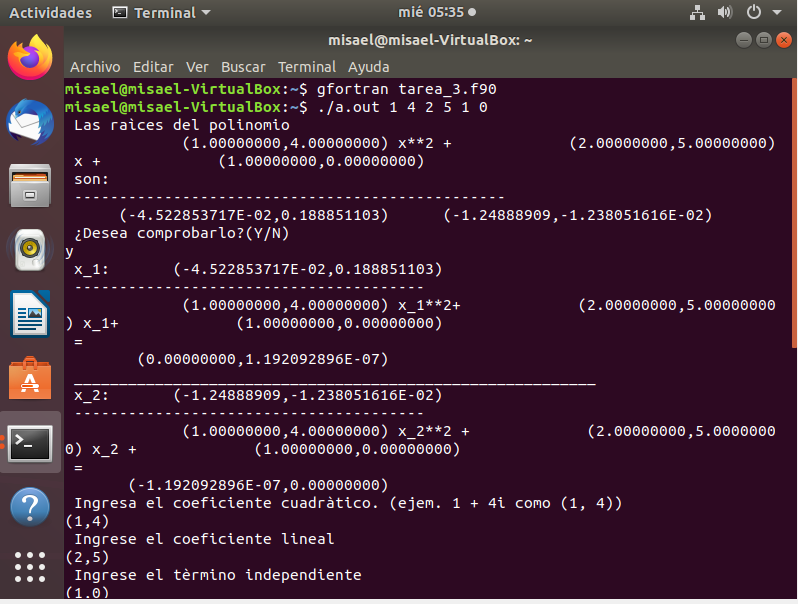
\includegraphics[scale = 0.7]{1.PNG}

\end{figure}

\begin{figure}[h!]
    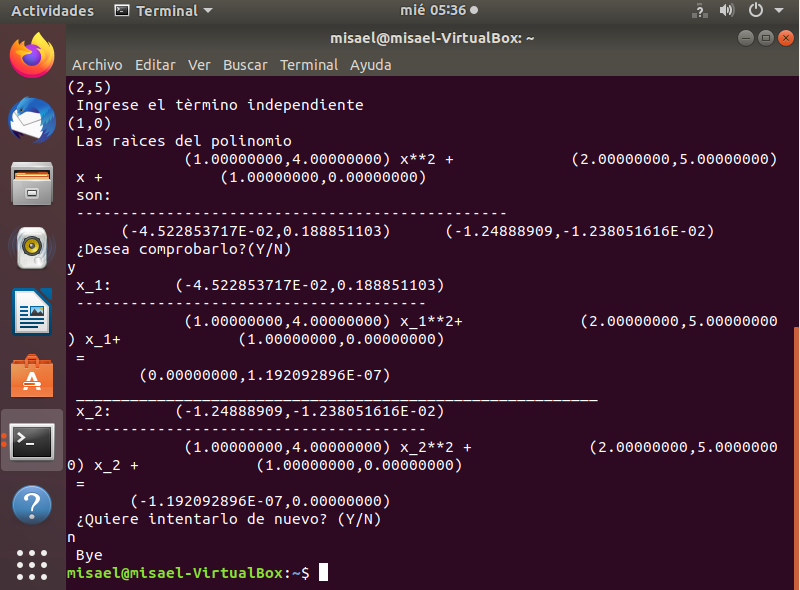
\includegraphics[scale = 0.7]{2.PNG}

\end{figure}



Los valores de la comprobación son muy cercanos al 0 y  arroja los mismos resultados que Wolfram así que debe estar bien

\begin{figure}
    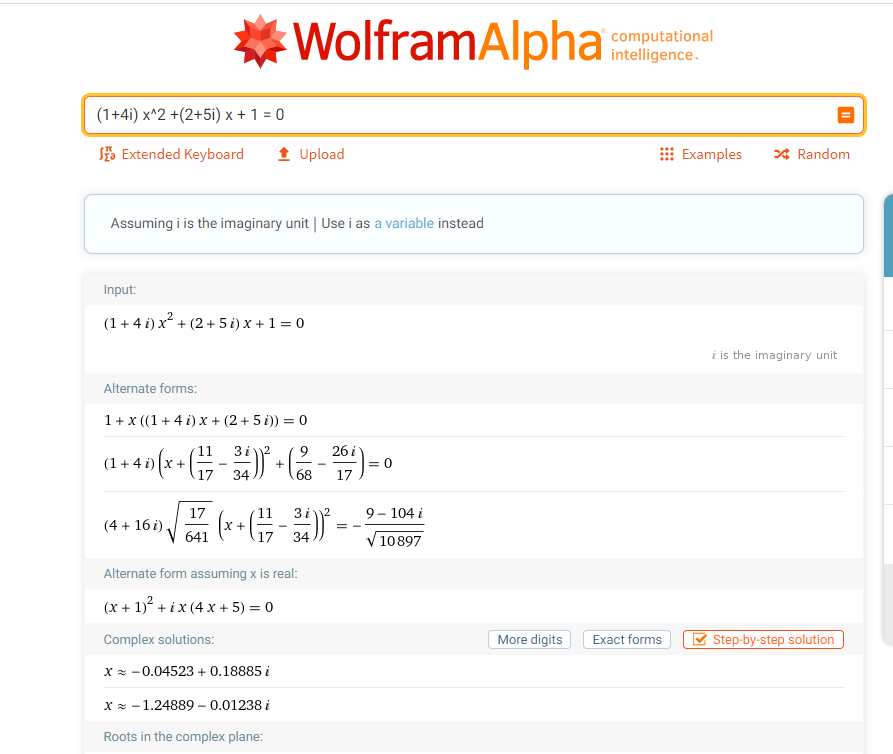
\includegraphics[scale = 0.7]{3.PNG}

\end{figure}
\end{document}